\newpage
\ReportSection{Operation Point %{{ op.id %}}}

\underline{\textsl{Operation Point \textbf}}\label}}}}
%{ include 'op_header.tex' %}

\vfill
%Plots
\begin{minipage}[t]{0.690\linewidth}
\textbf{Photon transfer plot}
\\*
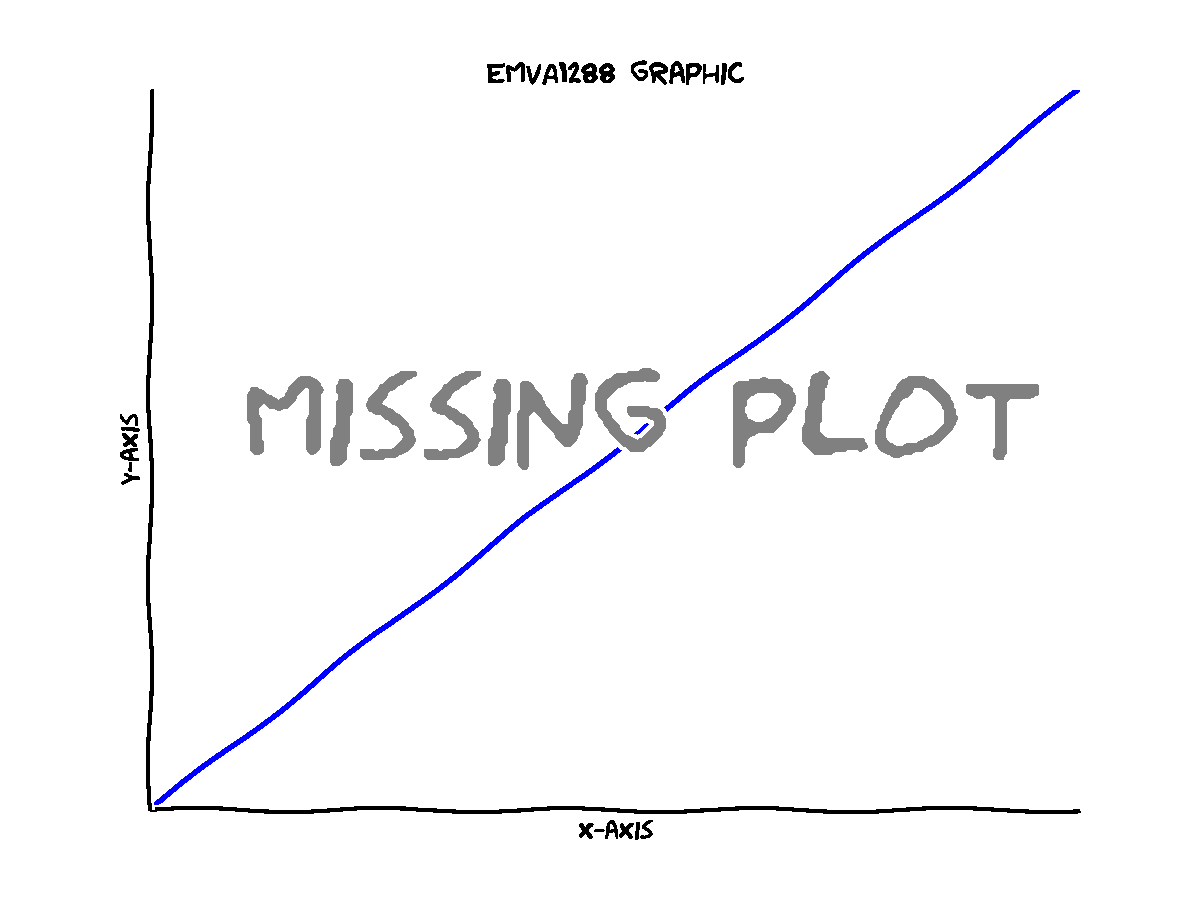
\includegraphics[width=0.95\linewidth,keepaspectratio]}}
\vfill
\textbf{Signal to noise ratio}
\\*
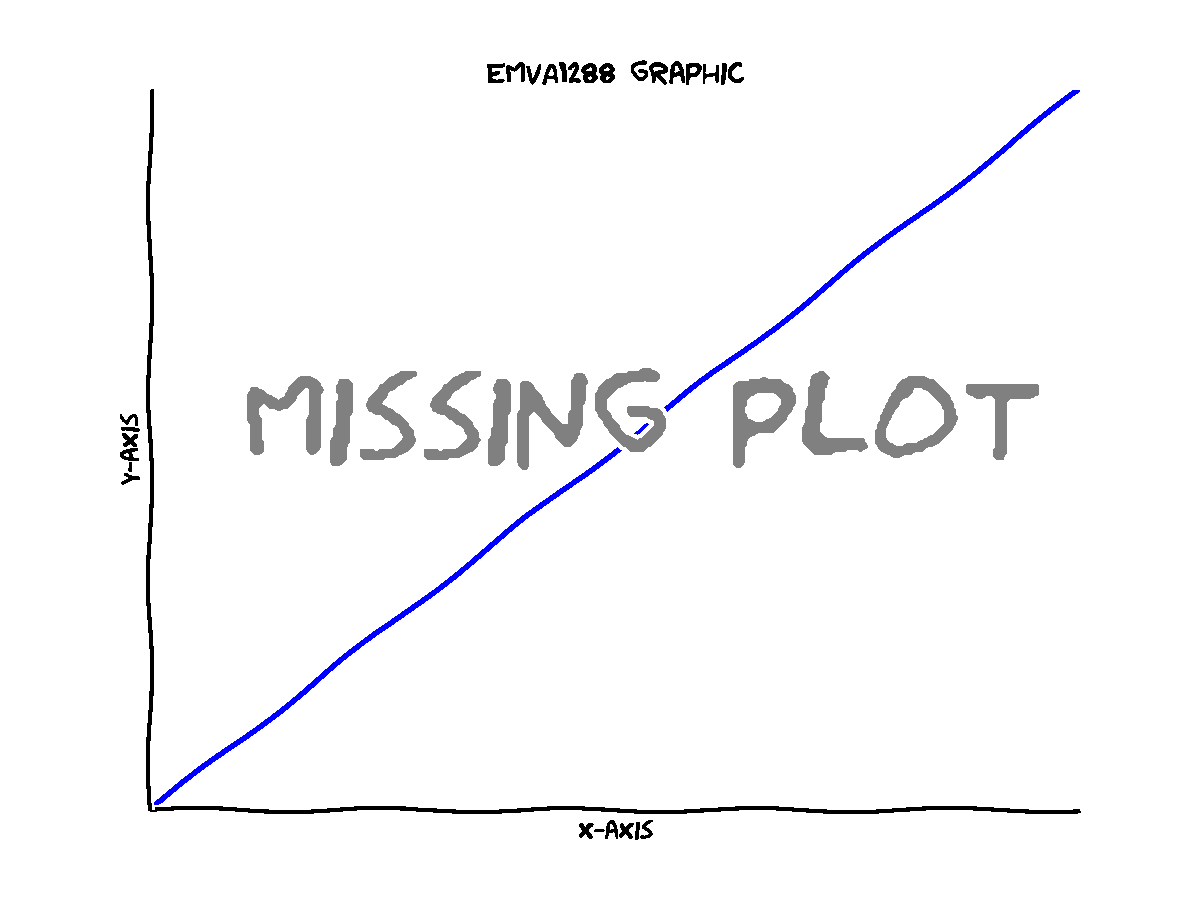
\includegraphics[width=0.95\linewidth,keepaspectratio]}}
\end{minipage}
%Results
\begin{minipage}[t]{0.290\linewidth}

\colorbox{greylight}{
\begin{minipage}[t]{0.975\linewidth}
\textsl{
%{{ op.results.sensitivity.QE.short %}}
(%{{ op.results.sensitivity.QE.unit %}})}
\hfill 
%{{ '%.2f' % op.results.sensitivity.QE.value %}}
\\[5mm]
\textsl{
%{{ op.results.sensitivity.K.short %}}
(%{{ op.results.sensitivity.K.unit %}})}
\hfill 
%{{ '%.3f' % op.results.sensitivity.K.value %}}
\\[1mm]
\textsl{
%{{ op.results.sensitivity.inverse_K.short %}}
(%{{ op.results.sensitivity.inverse_K.unit %}})}
\hfill 
%{{ '%.3f' % op.results.sensitivity.inverse_K.value %}}
\\[5mm]
\underline{\textbf{Noise:}}
\\*
\textsl{
%{{ op.results.sensitivity.sigma_y_dark.short %}}
(%{{ op.results.sensitivity.sigma_y_dark.unit %}})}
\hfill 
%{{ '%.3f' % op.results.sensitivity.sigma_y_dark.value %}}
\\[1mm]
\textsl{
%{{ op.results.sensitivity.sigma_d.short %}}
(%{{ op.results.sensitivity.sigma_d.unit %}})}
\hfill 
%{{ '%.3f' % op.results.sensitivity.sigma_d.value %}}
\\[3mm]
\textsl{
%{{ op.results.sensitivity.SNR_max.symbol %}}}
\hfill 
%{{ '%.3f' % op.results.sensitivity.SNR_max.value %}}
\\[1mm]
\textsl{
%{{ op.results.sensitivity.SNR_max_dB.symbol %}}
(%{{ op.results.sensitivity.SNR_max_dB.unit %}})}
\hfill 
%{{ '%.3f' % op.results.sensitivity.SNR_max_dB.value %}}
\\[1mm]
\textsl{
%{{ op.results.sensitivity.SNR_max_bit.symbol %}}
(%{{ op.results.sensitivity.SNR_max_bit.unit %}})}
\hfill 
%{{ '%.3f' % op.results.sensitivity.SNR_max_bit.value %}}
\\[1mm]
\textsl{
%{{ op.results.sensitivity.inverse_SNR_max.symbol %}}
(%{{ op.results.sensitivity.inverse_SNR_max.unit %}})}
\hfill 
%{{ '%.3f' % op.results.sensitivity.inverse_SNR_max.value %}}
\\[3mm]
\textsl{
%{{ op.results.sensitivity.u_p_min.short %}}
(%{{ op.results.sensitivity.u_p_min.unit %}})}
\hfill 
%{{ '%.3f' % op.results.sensitivity.u_p_min.value %}}
\\[1mm]
\textsl{
%{{ op.results.sensitivity.u_e_min.short %}}
(%{{ op.results.sensitivity.u_e_min.unit %}})}
\hfill 
%{{ '%.3f' % op.results.sensitivity.u_e_min.value %}}
\\[1mm]
\textsl{
%{{ op.results.sensitivity.u_p_sat.short %}}
(%{{ op.results.sensitivity.u_p_sat.unit %}})}
\hfill 
%{{ '%.0f' % op.results.sensitivity.u_p_sat.value %}}
\\[1mm]
\textsl{
%{{ op.results.sensitivity.u_e_sat.short %}}
(%{{ op.results.sensitivity.u_e_sat.unit %}})}
\hfill 
%{{ '%.0f' % op.results.sensitivity.u_e_sat.value %}}
\\[1mm]
\textsl{
%{{ op.results.sensitivity.DR.short %}}}
\hfill 
%{{ '%.0f' % op.results.sensitivity.DR.value %}}
\\[1mm]
\textsl{
%{{ op.results.sensitivity.DR_dB.short %}}
(%{{ op.results.sensitivity.DR_dB.unit %}})}
\hfill 
%{{ '%.1f' % op.results.sensitivity.DR_dB.value %}}
\\[1mm]
\textsl{
%{{ op.results.sensitivity.DR_bit.short %}}
(%{{ op.results.sensitivity.DR_bit.unit %}})}
\hfill 
%{{ '%.1f' % op.results.sensitivity.DR_bit.value %}}
\\[5mm]
\underline{\textbf{Spatial Nonuniformities:}}
\\*
\textsl{
%{{ op.results.spatial.DSNU1288.short %}}
(%{{ op.results.spatial.DSNU1288.unit %}})}
\hfill 
%{{ '%.1f' % op.results.spatial.DSNU1288.value %}}
\\[1mm]
\textsl{
%{{ op.results.spatial.DSNU1288_DN.short %}}
(%{{ op.results.spatial.DSNU1288_DN.unit %}})}
\hfill 
%{{ '%.1f' % op.results.spatial.DSNU1288_DN.value %}}
\\[1mm]
\textsl{
%{{ op.results.spatial.PRNU1288.short %}}
(%{{ op.results.spatial.PRNU1288.unit %}})}
\hfill 
%{{ '%.1f' % op.results.spatial.PRNU1288.value %}}
\\[5mm]
\underline{\textbf{Linearity:}}
\\*
\textsl{
%{{ op.results.linearity.LE_min.short %}}
(%{{ op.results.linearity.LE_min.unit %}})}
\hfill 
%{{ '%.3f' % op.results.linearity.LE_min.value %}}
\\[1mm]
\textsl{
%{{ op.results.linearity.LE_max.short %}}
(%{{ op.results.linearity.LE_max.unit %}})}
\hfill 
%{{ '%.3f' % op.results.linearity.LE_max.value %}}
\\[5mm]
\end{minipage}
}
\end{minipage}



%{ if op.extra %}
%Extra plots
\newpage
\begin{center}
\includegraphics[height=0.45\textheight,keepaspectratio]}}
\end{center}
\begin{center}
\includegraphics[height=0.45\textheight,keepaspectratio]}}
\end{center}
\vfill
\newpage
\begin{center}
\includegraphics[height=0.45\textheight,keepaspectratio]}}
\end{center}
\begin{center}
\includegraphics[height=0.45\textheight,keepaspectratio]}}
\end{center}
\vfill
\newpage
\begin{center}
\includegraphics[height=0.45\textheight,keepaspectratio]}}
\end{center}
\begin{center}
\includegraphics[height=0.45\textheight,keepaspectratio]}}
\end{center}
\vfill
\newpage
\begin{center}
\includegraphics[height=0.45\textheight,keepaspectratio]}}
\end{center}
\begin{center}
\includegraphics[height=0.45\textheight,keepaspectratio]}}
\end{center}
\vfill
\newpage
\begin{center}
\includegraphics[height=0.45\textheight,keepaspectratio]}}
\end{center}
\begin{center}
\includegraphics[height=0.45\textheight,keepaspectratio]}}
\end{center}
\vfill
\newpage
\begin{center}
\includegraphics[height=0.45\textheight,keepaspectratio]}}
\end{center}
\begin{center}
\includegraphics[height=0.45\textheight,keepaspectratio]}}
\end{center}
\vfill
\newpage
\begin{center}
\includegraphics[height=0.45\textheight,keepaspectratio]}}
\end{center}
\begin{center}
\includegraphics[height=0.45\textheight,keepaspectratio]}}
\end{center}
\vfill

%{ endif %}
